\documentclass{article}
\usepackage[utf8]{inputenc}
\usepackage[francais]{babel}
\usepackage[T1]{fontenc}
\usepackage{lmodern}
\usepackage{ifpdf}
\usepackage{pdflscape} % ou lscape
\usepackage{graphicx}
\renewcommand{\familydefault}{\sfdefault}

\title{Guidage des étudiants par GPS sur le Campus Triolet, UM2 - Android}
\author{PAGÈS Julien \and SALEIL Baptiste \and BENGHABRIT Walid}
\date{\today}
\ifpdf
	\pdfinfo 
	{
		/Author (Pagès - Saleil - Benghabrit)
		/Title (Guidage des étudiants par GPS sur le Campus Triolet, UM2 - Android)
		/Subject (Guidage des étudiants par GPS sur le Campus Triolet)
		/Keywords ()
		/CreationDate (\today)
	}
\fi

\begin{document}
	% Page de titre
	\maketitle
	\thispagestyle{empty}
	
	\section{Cahier des charges}
	Cette section présente un petit cahier des charges.
	Il présente les fonctionnalités que nous souhaitions développer pour l'application, et une exemple des différentes vues disponibles.
	
	\subsection{Caractéristiques}
	\begin{itemize}
		\item Interface simple, rapide, intuitive \\
			Le but ici est de fournir la meilleure expérience possible a l'utilisateur. Tout doit être accessible rapidement car l'application doit etre utilisée souvent, mais rapidement.
		\item Barre d'outils permettant de rechercher \\
			Lorsque l'application est lancée, l'utiliateur doit pouvoir effectuer une recherche en un clic. L'idéal serait de proposer une autocomplétion sur les résultats connus. La bare d'outils doit également proposer les préférences essentielles comme recentrer la carte sur l'utilisateur, etc...
		\item Carte affichée au lancement avec focus sur l'UM2 \\
			La carte doit être affichée au lancement de l'application de manière à ce que l'utilisateur soit tout de suite informé de sa position au sein de l'université si disponible, ou centré sur l'université sinon.
	\end{itemize}

	\subsection{Fonctionnalités}
	Ces fonctionnalités seront les premières implémentées car essentielles pour une telle application :
	\begin{itemize}
		\item Carte interactive
		\item Carte "annotée" avec les batiments, routes, etc...
		\item Liste brute des batiments ou l'utilisateur peut directement choisir son batiment.
		\item Guidage automatisé de l'utilisateur depuis sa position, vers la position souhaitée.
		\item Recherche textuelle / vocale permettant de rechercher un lieu le plus rapidement possible.
	\end{itemize}
	
	\subsection{Fonctionnalités souhaitées}
	Ces fonctionnalités seront implémentées si le temps nous le permet :
	\begin{itemize}
		\item Points clés (Cafétéria, parkings, ...) répertoriés par l'application pour enrichir son contenu.
		\item Guidage vocal de l'utilisateur
		\item Synchronisation avec l'emploi du temps ADE, l'utilisateur sélectionne son cursus et son groupe, et n'a plus qu'à lancer l'application pour connaitre sa salle et diriger.
		\item Mode "plus court" / "plus accessible" notamment pour les personnes handicapées, qui ne peuvent pas forcément emprunter les chemins de terre pour se rendre à un batiment.
	\end{itemize}
	
	\subsection{Vues}
	\begin{itemize}
	\item \textbf{Carte} : Affichage d'une carte en plein écran avec barre de menu pour préférences rapides. \\
	Voici une capture illustrant l'idée de notre application. Lorsque l'utilisateur lance l'application, la carte est l'élément affiché en premier. Une barre permet à l'utilisateur d'accéder aux fonctionnalités principales :  Recherche, Centrage,  etc... \\
		\begin{center}
			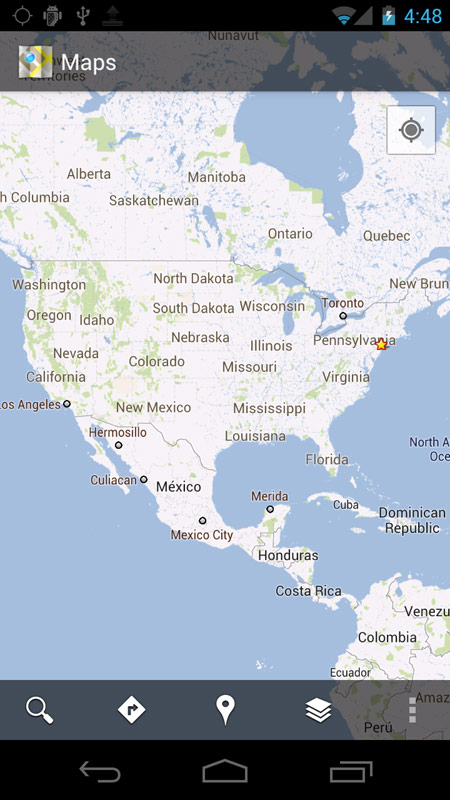
\includegraphics[scale=0.35]{map.jpg}
		\end{center}
	\item \textbf{Préférences} : Differents choix modifiant le comportement de l'application. \\
	La vue de présentation respectera le design et l'experience des menu classiques de préférences disponibles sur android avec cases à cocher ou autres widgets :
		\begin{center}
			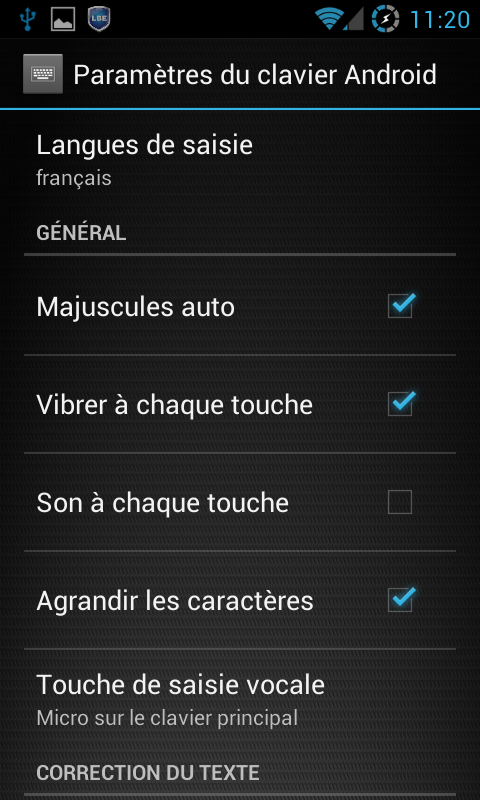
\includegraphics[scale=0.35]{preferences.png}
		\end{center}
	\item \textbf{Liste} : Choix lieu répertorié \\
	Cette vue permettra à l'utilisateur de parcourir l'ensemble des lieux répertoriés par l'application et éventuellement en choisir un.
	\end{itemize}
	
	\section{Réalisation}
	Dans cette section, nous allons présenter les différentes fonctionnalités que nous avons finalement développé pour cette application.
	
	% Carte
	\paragraph{Carte}
	Cette partie a été la première développée car c'est une fonctionnalité qui est à la base de toutes les autres. En effet, pour développer une application de guidage, l'affichage d'une carte est obligatoire. Soucieux de l'enjeu du logiciel libre, nous avons choisi de baser notre application sur \textit{OpenStreetMap} qui, de plus, est plus précise que \textit{Google Map} dans l'UM2. \\
	Afin que l'application soit accessible le plus rapidement possible, la carte est affiché dès le lancement de l'application : \\
	TODO
	
	% Recherche
	\paragraph{Recherche}
	Les deux premières icones sur la barre d'outils servent à la recherhce. Le premier ouvre la fenêtre de recherche textuelle. L'utilisateur peut alors rechercher un batiment ou un point d'interêt. Si un lieu est trouvé, le chemin est tracé. Sinon, l'utilisateur est notifié du fait que rien n'a été trouvé. \\
	Le deuxième correspond à la recherche vocale. Si l'utilisateur clique dessus, une fenêtre s'ouvre et il peut alors effectuer une recherche vocale. Par exemple, si on dit "Batiment 10" ou encore "Café" l'application va respectivement dessiner un chemin vers le batiment 10, ou afficher l'emplacement des machines à café. \\
	
	% GPS
	\paragraph{Guidage}
	L'application embarque un système de guidage de l'utilisateur. En effet, lorsque il recherche un batiment ou qu'il en sélectionne un, le chemin le plus court est dessiné entre sa position et le lieu sélectionné. De plus, l'utilisateur peut choisir dans les préférences d'activer le guidage vocal à la manière d'un GPS classique. \\
	Enfin, l'utilisateur peut cliquer sur le troisième bouton de la barre d'outils qui permet de centrer la vue sur sa position. \\
	
	% Liste
	\paragraph{Liste des lieux}
	Comme dit précédemment, l'utilisateur peut rechercher un batiment pour se faire guider. De plus, en cliquant sur l'icone "lieux" de la barre d'outils, il obtient une vue à trois onglets : \\
	\begin{itemize}
		\item \textbf{Batiments} : Cet onglet affiche une liste des batiments du campus Triolet. L'utilisateur peut cliquer dessus, et le guidage commence depuis sa position, vers le batiment sélectionné.
		\item \textbf{Planning} : Depuis les préférences, l'utilisateur peut importer un fichier ".ics" contenant son emploi du temps (fichier exportable depuis ADT). Dans cette vue, la liste des cours de la journée s'affichent. L'utilisateur peut cliquer sur l'un d'entre eux, et le guidage commencera entre sa position et le batiment ou a lieux le cours.
		\item \textbf{Autres} : Cet onglet affiche la liste des points d'interets de la fac. Si l'utilisateur clique dessus (par exemple café), des marqueurs vont s'afficher à chaque endroit ou se trouve une machine à café. L'utilisateur n'aura plus qu'a faire un clic long sur l'un d'entre eux pour démarrer le guidage.
	\end{itemize}
	
	% Préférences
	% Traduction
	% A propos
	
	\section{Conclusion}
		\subsection{Bilan}
		\subsection{difficultés}
	
\end{document}
